% IT5006 Phase 2 final report, version 3 (v2 analysis, teammates' v1 edits, short-promise drift findings).
% Run phase2_final/reports/phase2_final_evidence.py after updating saved results; it refreshes
% only the marked number and figure blocks below. This file compiles standalone.
\documentclass[12pt,a4paper]{article}
\usepackage[margin=0.8in]{geometry}
\usepackage[T1]{fontenc}
\usepackage{lmodern}
\usepackage{microtype}
\usepackage{booktabs}
\usepackage{array}
\usepackage{graphicx}
\usepackage{tikz}
\usepackage{float}
\usepackage{pgfplots}
\pgfplotsset{compat=1.16}
\usepackage{hyperref}
\hypersetup{colorlinks=true,linkcolor=blue,urlcolor=blue}
\setlength{\parindent}{0pt}
\setlength{\parskip}{0.4em}
\renewcommand{\arraystretch}{1.1}
% BEGIN GENERATED numbers -- refreshed by phase2_final_evidence.py
% Generated by reports/phase2_final_evidence.py: do not edit by hand.
\newcommand{\ActShare}{13}
\newcommand{\AllOrders}{96{,}272}
\newcommand{\AugModelNotPast}{79}
\newcommand{\AugRuleNotPast}{113}
\newcommand{\BadReviewLate}{62}
\newcommand{\BadReviewOnTime}{9}
\newcommand{\BadReviewRatio}{6.7}
\newcommand{\BenefitRatio}{5}
\newcommand{\BlackFridayLate}{12}
\newcommand{\BreakEvenRandomTest}{29}
\newcommand{\BreakEvenTest}{6.5}
\newcommand{\BreakEvenVal}{3.1}
\newcommand{\BusyGainMax}{28}
\newcommand{\BusyGainMin}{20}
\newcommand{\BusyRateMax}{21}
\newcommand{\BusyRateMin}{10}
\newcommand{\CalmGainMax}{25}
\newcommand{\CalmGainMin}{14}
\newcommand{\CalmRateMax}{5}
\newcommand{\CalmWindows}{W1 and W3}
\newcommand{\CarrierMean}{9.3}
\newcommand{\CarrierShare}{85}
\newcommand{\CheckoutBestMAE}{5.78}
\newcommand{\CheckoutBestName}{forest\_leaf20}
\newcommand{\CheckoutBestRMSE}{9.34}
\newcommand{\CheckoutBestRSq}{0.176}
\newcommand{\CheckoutImpAName}{numeric\_\_promised\_days}
\newcommand{\CheckoutImpAVal}{1.780}
\newcommand{\CheckoutImpBName}{logged\_\_distance\_km}
\newcommand{\CheckoutImpBVal}{1.111}
\newcommand{\CheckoutImpCName}{numeric\_\_route\_typical\_days}
\newcommand{\CheckoutImpCVal}{0.882}
\newcommand{\CheckoutImpKind}{coefficient (mean $|$weight$|$ over windows, numeric and engineered inputs; one-hot state/category dummies excluded from this ranking)}
\newcommand{\CheckoutMeanMAE}{7.21}
\newcommand{\CheckoutMeanRMSE}{10.67}
\newcommand{\CheckoutMeanRSq}{-0.078}
\newcommand{\CheckoutPR}{0.213}
\newcommand{\CheckoutRandTestMAE}{5.04}
\newcommand{\CheckoutRandTestRSq}{0.276}
\newcommand{\CheckoutRandValRSq}{0.259}
\newcommand{\CheckoutSelGap}{0.026}
\newcommand{\CheckoutSelGapSE}{0.028}
\newcommand{\CheckoutSelMAE}{5.81}
\newcommand{\CheckoutSelName}{ridge\_100}
\newcommand{\CheckoutSelRMSE}{9.40}
\newcommand{\CheckoutSelRSq}{0.167}
\newcommand{\CheckoutTestBias}{3.65}
\newcommand{\CheckoutTestMAE}{5.00}
\newcommand{\CheckoutTestRMSE}{6.41}
\newcommand{\CheckoutTestRSq}{-0.175}
\newcommand{\ClsBestName}{logistic\_c0.01}
\newcommand{\ClsCheckoutSelName}{logistic\_c0.01}
\newcommand{\ClsDefaultPR}{0.359}
\newcommand{\ClsNetBenefit}{-0.029}
\newcommand{\ClsPlainName}{logistic\_unregularized}
\newcommand{\ClsPlainPR}{0.354}
\newcommand{\ClsSelGap}{0.000}
\newcommand{\ClsSelGapSE}{0.000}
\newcommand{\ClsSelName}{logistic\_c0.01}
\newcommand{\ClsTestFone}{0.24}
\newcommand{\ClsTestLate}{3.5}
\newcommand{\ClsTestMCC}{0.25}
\newcommand{\ClsTestPR}{0.48}
\newcommand{\ClsTestPrec}{15.5}
\newcommand{\ClsTestROC}{0.85}
\newcommand{\ClsTestRec}{58}
\newcommand{\CohortOrders}{96{,}272}
\newcommand{\DisruptLateShare}{72}
\newcommand{\EtaTestOrders}{19{,}230}
\newcommand{\EtaTrainOrders}{75{,}039}
\newcommand{\ExcludedOrders}{198}
\newcommand{\FebMarLate}{17}
\newcommand{\FullDailyActiveDays}{81}
\newcommand{\FullDailyBeforePromise}{208}
\newcommand{\FullDailyCaught}{414}
\newcommand{\FullDailyCaughtOpen}{413}
\newcommand{\FullDailyCaughtPerDay}{5}
\newcommand{\FullDailyExpiredCaught}{206}
\newcommand{\FullDailyFlagged}{2{,}584}
\newcommand{\FullDailyLate}{705}
\newcommand{\FullDailyMedianFlagged}{36}
\newcommand{\FullDailyOrders}{19{,}534}
\newcommand{\FullDailyPninetyFlagged}{52}
\newcommand{\FullDailyPrecision}{16.0}
\newcommand{\FullDailyRecall}{58.7}
\newcommand{\FullDailyRecallRound}{59}
\newcommand{\GainFiveModel}{46}
\newcommand{\GainOneModel}{20}
\newcommand{\GainTenModel}{54}
\newcommand{\GainTwentyModel}{66}
\newcommand{\HandoverBestMAE}{5.10}
\newcommand{\HandoverBestName}{ridge\_100}
\newcommand{\HandoverBestRMSE}{8.41}
\newcommand{\HandoverBestRSq}{0.338}
\newcommand{\HandoverImpAName}{numeric\_\_handover\_days}
\newcommand{\HandoverImpAVal}{3.436}
\newcommand{\HandoverImpBName}{logged\_\_distance\_km}
\newcommand{\HandoverImpBVal}{1.218}
\newcommand{\HandoverImpCName}{numeric\_\_promise\_slack}
\newcommand{\HandoverImpCVal}{1.003}
\newcommand{\HandoverImpKind}{coefficient (mean $|$weight$|$ over windows, numeric and engineered inputs; one-hot state/category dummies excluded from this ranking)}
\newcommand{\HandoverMeanMAE}{7.21}
\newcommand{\HandoverMeanRMSE}{10.67}
\newcommand{\HandoverMeanRSq}{-0.078}
\newcommand{\HandoverRandTestMAE}{4.34}
\newcommand{\HandoverRandTestRSq}{0.411}
\newcommand{\HandoverRandValRSq}{0.386}
\newcommand{\HandoverRuleMAE}{5.30}
\newcommand{\HandoverRuleRSq}{0.337}
\newcommand{\HandoverSelGap}{0.000}
\newcommand{\HandoverSelGapSE}{0.000}
\newcommand{\HandoverSelMAE}{5.10}
\newcommand{\HandoverSelName}{ridge\_100}
\newcommand{\HandoverSelRMSE}{8.41}
\newcommand{\HandoverSelRSq}{0.338}
\newcommand{\HandoverTestBias}{2.87}
\newcommand{\HandoverTestMAE}{3.97}
\newcommand{\HandoverTestRMSE}{5.44}
\newcommand{\HandoverTestRSq}{0.154}
\newcommand{\ImpADrop}{0.088}
\newcommand{\ImpAName}{slack\_shortfall}
\newcommand{\ImpBDrop}{0.046}
\newcommand{\ImpBName}{handover\_days}
\newcommand{\ImpCDrop}{0.039}
\newcommand{\ImpCName}{remaining\_slack}
\newcommand{\ImpDDrop}{0.016}
\newcommand{\ImpDName}{distance\_km}
\newcommand{\ImpEDrop}{0.016}
\newcommand{\ImpEName}{route\_typical\_days}
\newcommand{\ImpFDrop}{0.014}
\newcommand{\ImpFName}{promised\_days}
\newcommand{\JunModelNotPast}{30}
\newcommand{\JunRuleNotPast}{30}
\newcommand{\LadderCheckoutMAE}{5.81}
\newcommand{\LadderCheckoutMinRSq}{0.060}
\newcommand{\LadderCheckoutRSq}{0.167}
\newcommand{\LadderElapsedMAE}{5.11}
\newcommand{\LadderElapsedMinRSq}{0.222}
\newcommand{\LadderElapsedRSq}{0.335}
\newcommand{\LadderHandoverMAE}{5.10}
\newcommand{\LadderHandoverMinRSq}{0.227}
\newcommand{\LadderHandoverRSq}{0.338}
\newcommand{\LadderTransitMAE}{5.68}
\newcommand{\LadderTransitMinRSq}{0.078}
\newcommand{\LadderTransitRSq}{0.214}
\newcommand{\LaterLift}{4.4}
\newcommand{\LaterLossPct}{9}
\newcommand{\LaterModelCaught}{387}
\newcommand{\LaterRuleCaught}{424}
\newcommand{\NormalLate}{4}
\newcommand{\OosGainPct}{12}
\newcommand{\OosModelCaught}{1{,}384}
\newcommand{\OosRuleCaught}{1{,}241}
\newcommand{\OosWins}{3}
\newcommand{\PastPromiseLateRate}{99.4}
\newcommand{\PastPromiseTest}{29.5}
\newcommand{\PastPromiseVal}{4.1}
\newcommand{\PastPromiseWinMax}{12}
\newcommand{\PastPromiseWinMin}{1}
\newcommand{\PrecFiveModel}{32}
\newcommand{\PrecOneModel}{70}
\newcommand{\PrecTenModel}{19}
\newcommand{\PrecTwentyModel}{12}
\newcommand{\PromAug}{15.2}
\newcommand{\PromJul}{19.7}
\newcommand{\PromJun}{27.8}
\newcommand{\PromSpanMax}{28}
\newcommand{\PromSpanMin}{22}
\newcommand{\RatedOrders}{95{,}627}
\newcommand{\RepeatAfterLate}{2.5}
\newcommand{\RepeatAfterOnTime}{3.0}
\newcommand{\RepeatShare}{3.0}
\newcommand{\RuleGapHigh}{0.062}
\newcommand{\RuleGapLow}{0.047}
\newcommand{\RuleGapPR}{0.054}
\newcommand{\RuleNetBenefit}{-0.020}
\newcommand{\RuleRecallTen}{59}
\newcommand{\RuleTestFone}{0.27}
\newcommand{\RuleTestPR}{0.52}
\newcommand{\RuleTestPrec}{16.9}
\newcommand{\RuleTestROC}{0.88}
\newcommand{\RuleTestRec}{63}
\newcommand{\RuleValPR}{0.328}
\newcommand{\ShapeBeatsRuleWindows}{5}
\newcommand{\ShapeRecallWith}{54}
\newcommand{\ShapeRecallWithout}{41}
\newcommand{\ShapeTestWith}{0.48}
\newcommand{\ShapeTestWithout}{0.23}
\newcommand{\ShapeValWith}{0.382}
\newcommand{\ShapeValWithout}{0.367}
\newcommand{\ShapeWinsWindows}{5}
\newcommand{\ShortCut}{14.5}
\newcommand{\ShortShareAug}{56}
\newcommand{\ShortTestPRModel}{0.146}
\newcommand{\ShortTestPRRule}{0.195}
\newcommand{\ShortValLateMax}{53}
\newcommand{\ShortValLateMin}{3}
\newcommand{\ShortValModelWins}{3}
\newcommand{\TestAugActed}{820}
\newcommand{\TestAugCaught}{234}
\newcommand{\TestAugLateCount}{393}
\newcommand{\TestAugOrders}{6{,}306}
\newcommand{\TestJulActed}{796}
\newcommand{\TestJulCaught}{119}
\newcommand{\TestJulLateCount}{207}
\newcommand{\TestJulOrders}{6{,}119}
\newcommand{\TestJunActed}{787}
\newcommand{\TestJunCaught}{33}
\newcommand{\TestJunLateCount}{70}
\newcommand{\TestJunOrders}{6{,}050}
\newcommand{\TestMayActed}{99}
\newcommand{\TestMayCaught}{1}
\newcommand{\TestMayLateCount}{2}
\newcommand{\TestMayOrders}{755}
\newcommand{\TestOrders}{19{,}230}
\newcommand{\TotalMean}{12.6}
\newcommand{\TrainPromised}{24.3}
\newcommand{\UniqueCustomers}{93{,}159}
\newcommand{\ValBestPR}{0.382}
\newcommand{\ValGainMax}{28}
\newcommand{\ValGainMin}{14}
\newcommand{\ValNetBenefit}{0.077}
\newcommand{\ValSelPR}{0.382}
\newcommand{\ValSelROC}{0.774}
\newcommand{\ValSelRecallTen}{36}
\newcommand{\WFiveModelCaught}{533}
\newcommand{\WFiveRuleCaught}{443}
\newcommand{\WTwoModelCaught}{401}
\newcommand{\WTwoRuleCaught}{313}
\newcommand{\WalkMaxGap}{0.003}
\newcommand{\WalkSame}{3}
% END GENERATED numbers

\begin{document}
\begin{titlepage}
\centering
\vspace*{0.8cm}
\IfFileExists{NUS_logo_full-horizontal.jpg}{%
  
\includegraphics[width=0.6\textwidth]{NUS_logo_full-horizontal.jpg}\par
}{%
  \IfFileExists{reports/NUS_logo_full-horizontal.jpg}{%
    \includegraphics[width=0.6\textwidth]{reports/NUS_logo_full-horizontal.jpg}\par
  }{%
    {\Huge\bfseries NUS\par}
    \vspace{0.2cm}
    {\large National University of Singapore\par}
    \vspace{1.8cm}
  }%
}
\vspace{1.6cm}
{\LARGE\bfseries Keeping Delivery Promises at Olist\par}
\vspace{0.4cm}
{\large Two-stage Delivery-time Estimation and Late-order Prioritisation at Carrier Handover\par}
\vspace{1.3cm}
{\large\bfseries IT5006 Phase 2\par}
\vspace{0.3cm}
{\large AY2026/27 Semester 1\par}
\vspace{1.4cm}
{\large\bfseries Group 6\par}
\vspace{0.6cm}
{\normalsize
CHAI WEI NI, WINNIE (A0172261M)\par
LE TRUNG HIEU (A0286973H)\par
LIANG ZIYAN (A0291506E)\par
LUM ZI YUAN JOSHUA (A0108499N)\par
SHAH PRATIK (A0211041H)\par
YUAN JIAYI (A0177893H)\par
}
\vfill
{\footnotesize Code and notebooks: \url{https://github.com/YuanJiayi/Team6_IT5006_Ecommerce_Analytics_AY2627Sem1}}\par
\vspace*{0.5cm}
\end{titlepage}

\section*{Executive Summary}
Late deliveries hurt Olist's reviews: \BadReviewLate{}\% of late orders receive a one- or two-star review, against \BadReviewOnTime{}\% of on-time orders. Our aim is to help the delivery operations team act on late orders early. When a seller hands a parcel to the carrier, two models help. The \textbf{classifier} ranks that day's parcels by their risk of missing the date the customer was promised. The \textbf{regression} estimates how many more days each delivery will take. Figure~\ref{fig:workflow} shows where both sit in an order's journey.

\begin{itemize}\setlength{\itemsep}{0pt}
\item \textbf{Delivery-time estimate.} Our chosen regression is a ridge regression ($\alpha=100$), selected on validation from four model families. At checkout it has an MAE of \CheckoutSelMAE{} days. Once the carrier has the parcel, we update the estimate using how long the order has already taken, and the MAE falls to \HandoverSelMAE{} days. The update is more accurate in every validation period, and it beats a simple rule of thumb, days so far plus the route's usual carrier time (MAE \HandoverRuleMAE{} days).
\item \textbf{Late warning.} Without a model, staff could rank parcels by their spare time: the days left until the promised date, minus how long the carrier usually takes on that route. A parcel promised in 6 days on a route that usually takes 8 has $-2$ days of spare time and goes near the top. Our chosen classifier, a regularised logistic regression ($C=0.01$) and the best of four model families on validation, produces a better list. Checking the same number of parcels, it finds \ValGainMin{}--\ValGainMax{}\% more late orders than this rule in every validation period.
\end{itemize}

Together, they give operations one daily list, produced while there is still time to act: which parcels to check first, and roughly when each will arrive.

\textbf{Final test period.} Over the most recent three months, the top 10\% of each month's parcels on the classifier's list held \GainTenModel{}\% of the late orders, more than five times what a random list would find. The spare-time rule did slightly better in this period, almost entirely because of data drift in August. That month Olist sharply shortened its promises, and \ShortShareAug{}\% of orders had promises under \ShortCut{} days, a length only one in ten training orders had. To respond to the drift, we tested retraining the model at the start of each month, instead of keeping the single model trained in May. It helped a little but could not catch up, because delivery outcomes arrive weeks late and the model can only learn from orders already delivered. The rule looks only at spare time, so it adapted at once. We therefore recommend a pilot that uses the classifier day to day, watches for data drift, and switches to the rule until the model has been properly retrained.

\section*{Business Problem and Model Roles}
\textbf{Why lateness matters.} Across \RatedOrders{} reviewed orders, late orders received a bad review (one or two stars) \BadReviewRatio{} times as often as on-time orders: \BadReviewLate{}\% against \BadReviewOnTime{}\%. Most of the uncertainty in delivery time comes from the carrier. The trip from handover to the customer takes \CarrierMean{} of the \TotalMean{} days an average order needs, and accounts for \CarrierShare{}\% of the variance in total delivery time (measured as its covariance share of that variance). Phase 1 also showed that delivery time grows with distance, from 5.9 days for the nearest sixth of orders to 18.5 for the furthest, and that a backlog lingered for weeks after the November sales peak. These findings shaped our distance and recent-history inputs.

\textbf{When to predict.} We predict at carrier handover. By then the parcel's progress is known, and the promised date is usually still ahead, so there is time to act. The classifier tells staff which orders to check first. The regression tells them how much longer each checked order is likely to take. We also fit the regression at checkout, before any progress is known, to show how much the handover information adds. We also tried using the regression to set the promised date itself, but it kept fewer promises than Olist's own dates in the busiest period (80.9\% on time against 86.2\%), so we keep Olist's date and focus on orders at risk of missing it.

\section*{Data Preparation and Evaluation Design}
From 99,441 Olist orders, 96,470 have both an actual and a promised delivery date. We drop \ExcludedOrders{} whose timestamps are out of order, such as a carrier handover recorded after delivery. That leaves \CohortOrders{} orders for both models. An order is \emph{late} if it arrives after the promised calendar date; arriving on the date counts as on time. Cancelled orders have no delivery date, so our results cover delivered orders only.

\textbf{One row per order.} We join orders to customers, items, products, sellers and payments, and combine item and payment rows so that each order appears once. For orders with several sellers, we use the furthest seller. Distance is the straight-line (Haversine) distance between the seller's and the customer's postcode areas, after removing 42 implausible coordinates; parcel-delivery studies use the same kind of distance~\cite{dearaujo2021}. Missing numbers are filled with the median of the training data only, and missing categories get their own ``unknown'' value. Repeat customers are counted with \texttt{customer\_unique\_id}, because \texttt{customer\_id} changes with every order.

\textbf{Evaluation design: learn from the past, test on the future.} A random split would let a model learn from orders delivered \emph{after} the ones it predicts, which is impossible in practice. It would also hide how conditions change over time~\cite{bergmeir2012}. We therefore split by date: a backtest over five validation windows, followed by a final test period.
\begin{itemize}\setlength{\itemsep}{0pt}
\item \textbf{Final test period:} the \TestOrders{} orders purchased from 26 May 2018, the most recent three months.
\item \textbf{Five validation windows} from 22 September 2017 to 26 March 2018, each with about 7,600 orders. For each window, the models learn only from orders purchased \emph{and delivered} before it starts, which is what Olist would have known at the time.
\item \textbf{A 60-day gap} before the final test period. Slow orders take weeks to arrive. Without the gap, the latest validation orders would include only the fast ones, and lateness would look lower than it really was.
\end{itemize}
We choose models on the five windows and use the final period to check the choice. The windows include both calm months and disruptions, so they also show how results vary with conditions. We looked at the final test period during development, so we treat it as a check on later conditions rather than a completely untouched test.

\textbf{Inputs and when they are known.} Phase 1 linked delivery time to the route, the timing of the order and its size. It also warned that information from later in an order's life must not leak into its own prediction. Table~\ref{tab:feature-rationale} lists each group of inputs, why we use it and when it becomes known.

\begin{table}[ht]
\centering\footnotesize
\caption{Model inputs, why we use them and when they are known. Every historical average uses only deliveries completed before the moment of prediction.}
\label{tab:feature-rationale}
\begin{tabular}{@{}p{2.25cm}p{6.25cm}p{7.15cm}@{}}
\toprule
Stage and input group & What it contains & Why, and its time boundary \\
\midrule
Checkout: route & Seller--customer distance; seller and customer state; the route's average past delivery time, pulled toward the overall average when a route has few orders. & Phase 1's distance finding and the use of historical transit times by Gibellini et al.~\cite{gibellini2024}; uses earlier Olist deliveries only. \\
Checkout: order & Purchase hour and weekday; item and seller counts; price, freight, weight and volume (log-scaled for linear models so a few very large orders do not dominate). & Salari et al. use order hour, weekday and item counts to forecast delivery time~\cite{salari2022}. \\
Checkout: promise & Days promised to the customer, and promised days minus the route's average delivery time. & Lateness is measured against this date. We \emph{assume} it was shown at checkout; the data has no record of promise changes. \\
Handover: progress & Days elapsed so far (and to payment approval); the route's average carrier time over the last 90 days; remaining slack, i.e.\ promised days minus elapsed days minus that carrier time. & Gibellini et al. use a shipment's observed progress and recent transit times~\cite{gibellini2024}. Only information known at handover; never this order's delivery. \\
Handover: slack shortfall & Whether the promised date had already passed at handover (yes/no); how many days slack is below zero (0 if positive). & Risk jumps once slack runs out. A logistic model treats slack as a straight line, so these inputs let it capture that jump; trees can split there without them. \\
\bottomrule
\end{tabular}
\end{table}

\textbf{Preventing leakage.} All preprocessing (filling gaps, encoding categories, scaling) runs inside scikit-learn pipelines, fitted on each window's training orders only. Route and seller histories use only orders already delivered when the prediction is made. No order's own delivery, review or later status is ever an input. Three inputs carry no history of when they were recorded: the promise, the payment details and the postcode map. That they were known at checkout is therefore an assumption. \textbf{Reproducibility.} The random seed (42), input list, split assignments and both model scripts are in \texttt{phase2\_final/} and reproduce every comparison. Appendix~\ref{app:gx} summarises separate data-quality checks.

\begin{figure}[ht]
\centering
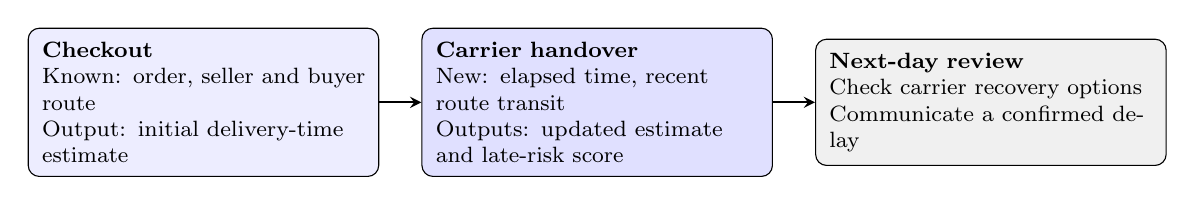
\begin{tikzpicture}[>=stealth,every node/.style={font=\footnotesize}]
\node[draw,rounded corners,fill=blue!7,align=left,text width=4.1cm,inner sep=5pt] (checkout) at (0,0) {\textbf{Checkout}\par Known: order, seller and buyer route\par Output: initial delivery-time estimate};
\node[draw,rounded corners,fill=blue!12,align=left,text width=4.1cm,inner sep=5pt] (handover) at (5.0,0) {\textbf{Carrier handover}\par New: elapsed time, recent route transit\par Outputs: updated estimate and late-risk score};
\node[draw,rounded corners,fill=gray!12,align=left,text width=4.1cm,inner sep=5pt] (action) at (10.0,0) {\textbf{Next-day review}\par Check carrier recovery options\par Communicate a confirmed delay};
\draw[->,thick] (checkout.east) -- (handover.west);
\draw[->,thick] (handover.east) -- (action.west);
\end{tikzpicture}
\caption{When each prediction is made and what follows. Lateness is judged against the date originally promised to the customer.}
\label{fig:workflow}
\end{figure}

\section*{Model 1: Two-stage Delivery-time Estimate (Regression)}
\textbf{Method.} Both stages predict total delivery days for the same orders. Subtracting the days already elapsed at handover gives the days still to go. The \textbf{checkout} model uses 20 inputs known at purchase, covering the order, route and seller. The \textbf{handover} model adds three inputs known once the carrier has the parcel: days elapsed since purchase, days to payment approval (if recorded by then), and the route's average carrier time over the previous 90 days. Table~\ref{tab:ladder} keeps the model fixed and adds this information one step at a time. Most of the gain comes from knowing how long the order has already taken.

\begin{table}[ht]
\centering\small
\caption{What each piece of information adds: the same ridge regression (\(\alpha=100\)) and the same orders at every step, mean over five validation windows.}
\label{tab:ladder}
\begin{tabular}{@{}lrrr@{}}
\toprule
Inputs & MAE (days) & \(R^2\) & Worst-window \(R^2\) \\
\midrule
Checkout (20 inputs) & \LadderCheckoutMAE{} & \LadderCheckoutRSq{} & \LadderCheckoutMinRSq{} \\
+ recent route transit history & \LadderTransitMAE{} & \LadderTransitRSq{} & \LadderTransitMinRSq{} \\
+ days elapsed to handover and approval & \LadderElapsedMAE{} & \LadderElapsedRSq{} & \LadderElapsedMinRSq{} \\
Handover model (route history updated to handover) & \LadderHandoverMAE{} & \LadderHandoverRSq{} & \LadderHandoverMinRSq{} \\
\bottomrule
\end{tabular}
\end{table}

\textbf{Candidates and selection.} We choose regression models by MAE, the average miss in days, because staff can use it directly; RMSE and $R^2$ are reported alongside. Each model family starts from its simplest version: the training average, plain linear regression and a single decision tree. More complex versions must beat these on validation to be kept: ridge regression, pruned trees, random forests and gradient boosting. At checkout, plain linear regression cuts the average miss from \CheckoutMeanMAE{} days (always predicting the average) to 5.86, and ridge to \CheckoutSelMAE{}. A single tree misses by 7.79 days and a random forest by \CheckoutBestMAE{}. At handover, ridge again leads at \HandoverSelMAE{} days; the forest improves on a single tree (6.84 to 5.35) but stays behind. A simple rule of thumb, days elapsed plus the route's recent carrier time, misses by \HandoverRuleMAE{} days. Knowing the days elapsed therefore gives most of the gain, and the model adds a further 0.2 days by weighing order and route details.

When two models are close, we prefer the simpler one. A more complex model must win by more than the typical window-to-window variation in the gap between them (the one-standard-error rule~\cite{james2013}). At checkout the forest beats ridge by only \CheckoutSelGap{} days, inside that variation (\CheckoutSelGapSE{}), so we choose ridge ($\alpha=100$). At handover, ridge is the most accurate outright. An ensemble that averages ridge and boosting misses by 5.11 days, no better than ridge alone. Every candidate is in Appendix Table~\ref{tab:app-regression}.

\begin{figure}[ht]
\centering
% BEGIN GENERATED fig_ladder -- refreshed by phase2_final_evidence.py
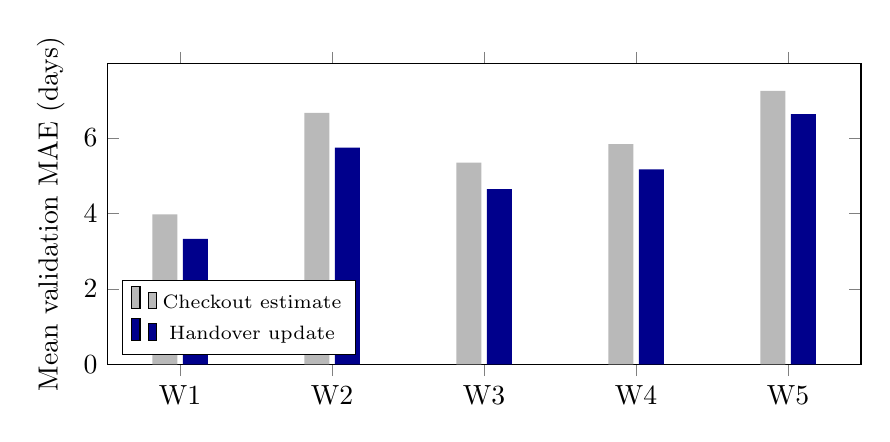
\begin{tikzpicture}
\begin{axis}[width=0.92\linewidth,height=5.4cm,ybar,bar width=9pt,ymin=0,ylabel={Mean validation MAE (days)},
 symbolic x coords={W1,W2,W3,W4,W5},xtick=data,enlarge x limits=0.12,legend style={at={(0.02,0.03)},anchor=south west,font=\scriptsize}]
\addplot[fill=gray!55,draw=none] coordinates {(W1,3.97) (W2,6.66) (W3,5.34) (W4,5.83) (W5,7.24)};
\addplot[fill=blue!55!black,draw=none] coordinates {(W1,3.32) (W2,5.74) (W3,4.64) (W4,5.16) (W5,6.63)};
\legend{Checkout estimate,Handover update}
\end{axis}
\end{tikzpicture}
% END GENERATED fig_ladder
\caption{MAE in each validation window: the checkout estimate against the handover update. The handover update is more accurate in every window, including the high-lateness ones.}
\label{fig:ladder}
\end{figure}

\textbf{Final test period.} The handover update still cuts the average miss by about a day: \HandoverTestMAE{} days against \CheckoutTestMAE{} at checkout (RMSE \HandoverTestRMSE{} against \CheckoutTestRMSE{}). However, deliveries in this period were faster than in the training data, and both models predicted too long, by \CheckoutTestBias{} and \HandoverTestBias{} days on average (Appendix Figure~\ref{fig:test-bias}). The same shift explains the negative checkout $R^2$ (\CheckoutTestRSq{}; handover \HandoverTestRSq{}): $R^2$ compares the model with the period's own, unusually low, average. We therefore show the estimate to staff as guidance, not as a new date for the customer, and track this bias monthly. For comparison, a random split of the same orders gives the handover model an $R^2$ of \HandoverRandTestRSq{}, against \HandoverSelRSq{} across the time-ordered windows; the gap reflects changing delivery conditions, not a different model, which is why we do not rely on random-split scores (Appendix~\ref{app:diag}).

\textbf{What drives the estimate.} With inputs standardised, the largest ridge coefficients at checkout belong to promised days (\CheckoutImpAVal{}), distance (\CheckoutImpBVal{}) and the route's typical delivery time (\CheckoutImpCVal{}). At handover, days elapsed dominates (\HandoverImpAVal{}), as Table~\ref{tab:ladder} suggests. The inputs are correlated, so these coefficients describe what the model relies on, not cause and effect.

\section*{Model 2: The Late Warning (Classification)}
\textbf{Candidates and selection.} Each family again starts simple: plain logistic regression scores a validation PR-AUC of \ClsPlainPR{}, and a single tree 0.137. We then try regularisation, class weighting, pruned trees, random forests and gradient boosting (Table~\ref{tab:family-summary}; every configuration is in Appendix Table~\ref{tab:app-classifier}). Logistic regression with strong regularisation ($C=0.01$) scores best, at \ValSelPR{}. Giving extra weight to the rare late orders lowers its score to 0.372, so we keep their natural share. The best random forest also reaches 0.372. It trails logistic regression by more than the window-to-window variation (0.011 against 0.004), so logistic regression wins outright. The choice is also stable: choosing on earlier windows only, the same model comes out ahead before each of the last three windows, never more than \WalkMaxGap{} below the best candidate there.

% BEGIN GENERATED fig_family_summary -- refreshed by phase2_final_evidence.py
\begin{table}[ht]
\centering\small
\caption{Classifiers by family, mean over five validation windows: the simplest version of each family and its best tuned version, against the remaining-slack rule. Every configuration is in Appendix Table~\ref{tab:app-classifier}.}
\label{tab:family-summary}
\begin{tabular}{@{}llrrr@{}}
\toprule
Family & Configuration & PR-AUC & ROC-AUC & Recall at top 10\% \\
\midrule
Linear & logistic\_unregularized (simplest) & 0.354 & 0.736 & 34\% \\
Linear & logistic\_c0.01 (best tuned) & 0.382 & 0.774 & 36\% \\
Tree & tree\_plain (simplest) & 0.137 & 0.559 & 21\% \\
Tree & tree\_d8\_l100 (best tuned) & 0.308 & 0.684 & 32\% \\
Forest & forest\_l50\_sqrt (best tuned) & 0.372 & 0.750 & 34\% \\
Boosting & boost\_lr0.03\_n200\_l20 (best tuned) & 0.356 & 0.743 & 33\% \\
Rule & remaining slack (benchmark) & 0.328 & 0.697 & 30\% \\
\bottomrule
\end{tabular}
\end{table}
% END GENERATED fig_family_summary

\textbf{Benchmark: the remaining-slack rule.} Without any model, staff could sort parcels by remaining slack: the days left before the promised date, minus the route's recent carrier time. A model is only worth deploying if it beats this rule. Ours does on validation, with a PR-AUC of \ValSelPR{} against \RuleValPR{} and a win in all five windows. The 95\% bootstrap interval for the gap runs from \RuleGapLow{} to \RuleGapHigh{}, well clear of zero.

Two inputs are essential to this result: whether the promised date has already passed, and by how many days slack has run out. An order already past its date at handover is almost certainly late (\PastPromiseLateRate{}\% were, in validation). But a logistic model treats slack as a straight line and cannot express that jump on its own. Without these inputs, the model scores \ShapeValWithout{} on validation, and its final-test score halves from \ShapeTestWith{} to \ShapeTestWithout{}. We added them after the final test period showed the rule doing better. We kept them because they improve every validation window, not because of the test result.

\textbf{Handling imbalance.} Late orders are rare: \ClsTestLate{}\% in the final test period and 4--21\% across the validation windows. Accuracy would therefore mislead, because predicting ``on time'' for every order would score highly. We choose models by PR-AUC, which focuses on the late orders, and show each period's late rate as the score a random list would get~\cite{saito2015}. We also report ROC-AUC, and precision, recall and F1 for a review list of fixed size. Curves, and confusion counts with MCC, are in the appendix (Figure~\ref{fig:roc-pr}, Table~\ref{tab:app-confusion}).

Table~\ref{tab:classifier-windows} shows why a single average is not enough. The late rate swings from 4\% to 21\% between windows, and the precision of the top 10\% swings with it. Yet that precision always beats the late rate, and ROC-AUC stays between 0.75 and 0.81. The model finds late orders in calm and busy periods alike; what changes is how many there are to find.

% BEGIN GENERATED fig_classifier_windows -- refreshed by phase2_final_evidence.py
\begin{table}[ht]
\centering\small
\caption{The selected classifier in each validation window. The late rate of each window is the PR-AUC of a random list.}
\label{tab:classifier-windows}
\begin{tabular}{@{}lrrrrr@{}}
\toprule
Window & Orders & Late rate & PR-AUC & ROC-AUC & Top-10\% precision \\
\midrule
W1 & 7,600 & 4.1\% & 0.374 & 0.811 & 20.8\% \\
W2 & 7,601 & 13.8\% & 0.416 & 0.768 & 43.8\% \\
W3 & 7,601 & 4.8\% & 0.281 & 0.750 & 16.6\% \\
W4 & 7,601 & 9.9\% & 0.356 & 0.780 & 34.6\% \\
W5 & 7,600 & 20.7\% & 0.483 & 0.759 & 57.2\% \\
\bottomrule
\end{tabular}
\end{table}
% END GENERATED fig_classifier_windows

\textbf{Final test period.} The model's PR-AUC is \ClsTestPR{}, against \ClsTestLate{}\% for a random list, and its ROC-AUC is \ClsTestROC{}. Ranking the orders of each purchase month, the top 10\% contains \GainTenModel{}\% of that month's late orders, more than five times what a random list would find (Figure~\ref{fig:gains}).

\textbf{Value across periods.} Table~\ref{tab:period-value} compares the model with the rule in every period, with both checking the same number of orders. The model finds more late orders in all five validation windows. Its advantage does not depend on deliveries going badly: it finds \CalmGainMin{}\% and \CalmGainMax{}\% more in the calm windows (\CalmWindows{}) and \BusyGainMin{}--\BusyGainMax{}\% more in the busy ones. In absolute numbers the gains are largest in the busy windows, because they contain more late orders: \WTwoModelCaught{} against \WTwoRuleCaught{} around Black Friday (W2), and \WFiveModelCaught{} against \WFiveRuleCaught{} in February--March (W5).

The one exception is the final test period, where the rule finds slightly more late orders (\LaterRuleCaught{} against \LaterModelCaught{}). Both rankings put every parcel already past its promised date at the top, so the difference lies in parcels that still had time, and almost all of it arose in August. In June the two found the same number of these late parcels (\JunModelNotPast{}); in August the rule found \AugRuleNotPast{} and the model \AugModelNotPast{}.

August stands out because the data drifted away from what the model had learned. From March 2017 to May 2018 the monthly average promise stayed between \PromSpanMin{} and \PromSpanMax{} days. In August it fell to \PromAug{}, and \ShortShareAug{}\% of orders had promises under \ShortCut{} days, the shortest tenth of training promises. The model had never been clearly better than the rule on such orders. In validation it was ahead in \ShortValModelWins{} of the five windows, each with only \ShortValLateMin{}--\ShortValLateMax{} short-promise late orders to learn from, and in the final period the rule ranked them clearly better (PR-AUC \ShortTestPRRule{} against \ShortTestPRModel{}). Once these orders made up most of August, the model lost its edge.

Even so, across the four periods evaluated after the model was chosen (W3--W5 and the final period), the model finds \OosModelCaught{} late orders against the rule's \OosRuleCaught{}, \OosGainPct{}\% more, and wins three of the four.

\textbf{Responding to the drift.} We tested three remedies, each compared on the validation windows first (Appendix~\ref{app:remedies}). Retraining every month found 5\% more late orders than retraining every quarter on validation, and 3\% more than the single frozen model in the final period, but still trailed the rule in August. Removing the raw promise inputs changed almost nothing, because promise length can be rebuilt exactly from spare time, days elapsed and the route's carrier time. A rule-first model, allowed only to adjust the spare-time score, caught as many late orders as the current model on validation but did no better in August. All three run into the same limit: the model learns only from delivered orders, and on 1 August only about one in ten orders with known outcomes had a short promise. The rule needs no history, which is why it is the right backup when promises change.

% BEGIN GENERATED fig_period_value -- refreshed by phase2_final_evidence.py
\begin{table}[ht]
\centering\small
\caption{Model against the remaining-slack rule at the same workload: the top \ActShare{}\% of each window, or of each purchase month in the final test period (Later). W3--W5 and the final test period were evaluated after the model was chosen on earlier windows. A random list would catch \ActShare{}\% of late orders.}
\label{tab:period-value}
\begin{tabular}{@{}lrrrrrrr@{}}
\toprule
& & Late already & \multicolumn{2}{c}{PR-AUC} & \multicolumn{3}{c}{Late orders caught} \\
\cmidrule(lr){4-5}\cmidrule(l){6-8}
Period & Late rate & past date & Model & Rule & Model & Rule & Random \\
\midrule
W1 & 4.1\% & 12\% & 0.374 & 0.354 & 175 & 153 & 40 \\
W2 & 13.8\% & 6\% & 0.416 & 0.343 & 401 & 313 & 137 \\
W3 & 4.8\% & 7\% & 0.281 & 0.256 & 146 & 117 & 47 \\
W4 & 9.9\% & 3\% & 0.356 & 0.301 & 318 & 257 & 98 \\
W5 & 20.7\% & 1\% & 0.483 & 0.386 & 533 & 443 & 205 \\
Later & 3.5\% & 29\% & 0.477 & 0.519 & 387 & 424 & 87 \\
\bottomrule
\end{tabular}
\end{table}
% END GENERATED fig_period_value

\textbf{Size of the review list.} We compared lists covering 1\% to 30\% of handovers. With no cost data, we assumed that finding a late order is worth \BenefitRatio{} times the cost of one review. Under that assumption, the best list size on validation is \ActShare{}\%. The answer depends heavily on the assumption, though: a ratio of two would pick 1\%, and a ratio of ten would pick 30\%. A list sized for a busy season can also overspend in a quieter one. List size is therefore a business decision, and we show below how to make it without the assumption.

For simplicity, this comparison picks the top orders from each whole window or purchase month, which uses scores from later in that month. The daily replay below does it day by day, as operations would.

\begin{table}[ht]
\centering\small
\caption{Final test period: ranking quality and the top-\ActShare{}\% review list within each purchase month. PR-AUC and ROC-AUC use all orders; precision, recall and F1 use the review list.}
\label{tab:classifier-test}
\begin{tabular}{@{}lccccc@{}}
\toprule
& PR-AUC & ROC-AUC & Precision & Recall & F1 \\
\midrule
Late-warning model & \ClsTestPR{} & \ClsTestROC{} & \ClsTestPrec{}\% & \ClsTestRec{}\% & \ClsTestFone{} \\
Remaining-slack rule & \RuleTestPR{} & \RuleTestROC{} & \RuleTestPrec{}\% & \RuleTestRec{}\% & \RuleTestFone{} \\
Random list & \ClsTestLate{}\% & 0.50 & \ClsTestLate{}\% & \ActShare{}\% & --- \\
\bottomrule
\end{tabular}
\end{table}

\textbf{What the review list is worth.} The cost ratio of five is our assumption, so we also show the result without it. Each order on the list costs one check. At the \ActShare{}\% list size, about 1 in \BreakEvenVal{} listed orders was late in the validation periods and 1 in \BreakEvenTest{} in the calm final period, against 1 in \BreakEvenRandomTest{} for a random list there (Table~\ref{tab:classifier-test}). The list therefore pays off whenever rescuing a late order is worth more than about three checks in busy periods, or six to seven in calm ones. At the assumed ratio of five, it earns \ValNetBenefit{} per order on validation but falls just short in the final period (\ClsNetBenefit{}; the rule \RuleNetBenefit{}), when only \ClsTestLate{}\% of orders were late. A shorter list is more efficient: in the final period, \PrecFiveModel{}\% of the top 5\% were late. Operations should set the list length from the measured cost of a check and value of a rescue, and lengthen it when lateness rises. Monthly counts are in Appendix Table~\ref{tab:classifier-monthly}.

\textbf{Daily replay.} To check the workload in practice, we replayed the model day by day over the final test period, flagging the top \ActShare{}\% of each day's handovers. This flagged a median of \FullDailyMedianFlagged{} orders a day. Of \FullDailyLate{} late orders, it found \FullDailyCaught{} (\FullDailyRecall{}\% recall, \FullDailyPrecision{}\% precision). By 9am the next morning, \FullDailyBeforePromise{} of the late orders found were still before their promised date, so there was time to act. The other \FullDailyExpiredCaught{} had already missed it and call for an update to the customer instead (Appendix Table~\ref{tab:daily-replay}).

% BEGIN GENERATED fig_split_summary -- refreshed by phase2_final_evidence.py
\begin{table}[ht]
\centering\small
\caption{Chosen models on training data, validation (mean of five windows) and the final test period. The periods differ in late rate.}
\label{tab:split-summary}
\begin{tabular}{@{}lrrr@{}}
\toprule
Metric & Training & Validation & Final test \\
\midrule
Checkout MAE (days) & 5.23 & 5.81 & 5.00 \\
Handover MAE (days) & 4.57 & 5.10 & 3.97 \\
Late warning PR-AUC & 0.344 & 0.382 & 0.477 \\
Late prevalence & 7.1\% & 10.7\% & 3.5\% \\
\bottomrule
\end{tabular}
\end{table}
% END GENERATED fig_split_summary

Table~\ref{tab:split-summary} puts the chosen models side by side across training, validation and the final test period. The handover model beats the checkout model in all three. The classifier scores higher in the final period than in validation (PR-AUC \ClsTestPR{} against \ValSelPR{}), even though fewer orders were late. This is largely because more of the final period's late orders had already missed their date, which makes them easy to rank. Training scores are measured on the data the models learned from and are shown for reference only.

\begin{figure}[ht]
\centering
% BEGIN GENERATED fig_gains -- refreshed by phase2_final_evidence.py
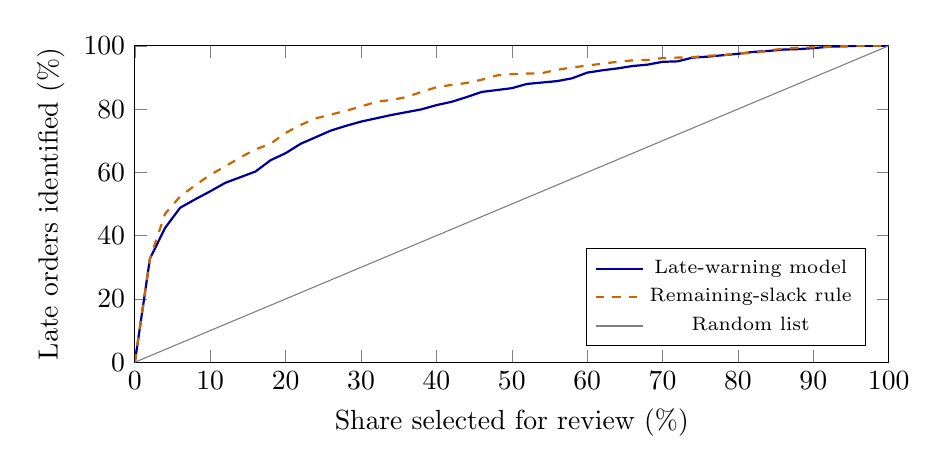
\begin{tikzpicture}
\begin{axis}[width=0.92\linewidth,height=5.6cm,xlabel={Share selected for review (\%)},ylabel={Late orders identified (\%)},
 xmin=0,xmax=100,ymin=0,ymax=100,legend style={at={(0.97,0.05)},anchor=south east,font=\scriptsize}]
\addplot[thick,blue!60!black,no marks] coordinates {(0.0,0.0000) (2.0,32.7381) (4.0,42.4107) (6.0,48.8095) (8.0,51.4881) (10.0,54.0179) (12.0,56.6964) (14.000000000000002,58.4821) (16.0,60.2679) (18.0,63.8393) (20.0,66.0714) (22.0,69.0476) (24.0,71.1310) (26.0,73.2143) (28.000000000000004,74.7024) (30.0,76.0417) (32.0,77.0833) (34.0,78.1250) (36.0,79.0179) (38.0,79.9107) (40.0,81.2500) (42.0,82.2917) (44.0,83.7798) (46.0,85.4167) (48.0,86.0119) (50.0,86.6071) (52.0,87.9464) (54.0,88.3929) (56.00000000000001,88.8393) (57.99999999999999,89.7321) (60.0,91.5179) (62.0,92.2619) (64.0,92.8571) (66.0,93.6012) (68.0,94.0476) (70.0,94.9405) (72.0,95.0893) (74.0,96.2798) (76.0,96.5774) (78.0,97.0238) (80.0,97.4702) (82.0,98.0655) (84.0,98.3631) (86.0,98.8095) (88.0,98.9583) (90.0,99.2560) (92.0,99.7024) (94.0,99.8512) (96.0,100.0000) (98.0,100.0000) (100.0,100.0000)};
\addlegendentry{Late-warning model}
\addplot[thick,orange!80!black,dashed,no marks] coordinates {(0.0,0.0000) (2.0,32.7381) (4.0,46.8750) (6.0,52.3810) (8.0,55.9524) (10.0,59.2262) (12.0,61.9048) (14.000000000000002,64.7321) (16.0,67.2619) (18.0,69.0476) (20.0,72.4702) (22.0,75.0000) (24.0,77.0833) (26.0,78.2738) (28.000000000000004,79.4643) (30.0,80.8036) (32.0,82.2917) (34.0,82.8869) (36.0,83.7798) (38.0,85.4167) (40.0,86.9048) (42.0,87.6488) (44.0,88.2440) (46.0,89.2857) (48.0,90.6250) (50.0,91.0714) (52.0,91.2202) (54.0,91.3690) (56.00000000000001,92.4107) (57.99999999999999,93.1548) (60.0,93.7500) (62.0,94.3452) (64.0,94.9405) (66.0,95.3869) (68.0,95.5357) (70.0,96.1310) (72.0,96.2798) (74.0,96.4286) (76.0,96.8750) (78.0,97.0238) (80.0,97.6190) (82.0,97.6190) (84.0,98.5119) (86.0,99.1071) (88.0,99.4048) (90.0,99.5536) (92.0,99.7024) (94.0,99.8512) (96.0,100.0000) (98.0,100.0000) (100.0,100.0000)};
\addlegendentry{Remaining-slack rule}
\addplot[thin,gray,no marks] coordinates {(0.0,0.0000) (2.0,2.0000) (4.0,4.0000) (6.0,6.0000) (8.0,8.0000) (10.0,10.0000) (12.0,12.0000) (14.000000000000002,14.0000) (16.0,16.0000) (18.0,18.0000) (20.0,20.0000) (22.0,22.0000) (24.0,24.0000) (26.0,26.0000) (28.000000000000004,28.0000) (30.0,30.0000) (32.0,32.0000) (34.0,34.0000) (36.0,36.0000) (38.0,38.0000) (40.0,40.0000) (42.0,42.0000) (44.0,44.0000) (46.0,46.0000) (48.0,48.0000) (50.0,50.0000) (52.0,52.0000) (54.0,54.0000) (56.00000000000001,56.0000) (57.99999999999999,58.0000) (60.0,60.0000) (62.0,62.0000) (64.0,64.0000) (66.0,66.0000) (68.0,68.0000) (70.0,70.0000) (72.0,72.0000) (74.0,74.0000) (76.0,76.0000) (78.0,78.0000) (80.0,80.0000) (82.0,82.0000) (84.0,84.0000) (86.0,86.0000) (88.0,88.0000) (90.0,90.0000) (92.0,92.0000) (94.0,94.0000) (96.0,96.0000) (98.0,98.0000) (100.0,100.0000)};
\addlegendentry{Random list}
\end{axis}
\end{tikzpicture}
% END GENERATED fig_gains
\caption{Share of late orders caught against share of orders reviewed, final test period, ranking within each purchase month.}
\label{fig:gains}
\end{figure}

\textbf{What drives the score.} We shuffled one input at a time and measured how much validation PR-AUC dropped~\cite{breiman2001}. The most important inputs are slack shortfall (\ImpADrop{}), days elapsed (\ImpBDrop{}) and remaining slack (\ImpCDrop{}); every other input matters less than 0.02. The model mainly reads how far an order has fallen behind its promised date, which only becomes visible at handover.

\section*{Proposed Operations Workflow}
\begin{enumerate}\setlength{\itemsep}{0pt}
\item \textbf{Each day at handover}, score every new parcel for late risk against its promised date and estimate its remaining delivery time. Rank the day's parcels for review the next morning. If the model is unavailable, rank by remaining slack instead.
\item \textbf{Each morning}, staff check the top of the list, up to a capacity operations chooses, with the remaining-time estimate to hand. Orders already past their date get an immediate update to the customer. For the rest, staff ask the carrier whether a faster service or another recovery option exists, and at what cost.
\item \textbf{Each month}, track whether the delivery estimate runs consistently long or short, the late rate, the length of Olist's promises, and how many flagged orders turn out late. A sustained change, or a change in how Olist sets promises, is the signal to retrain the models or resize the list. If the data drifts sharply, as promise lengths did in August 2018, switch to the rule until the model has been retrained on enough of the new orders. The pilot should test this switch, since we designed it after seeing August.
\end{enumerate}

\section*{Limitations and Pilot Requirements}
\begin{itemize}\setlength{\itemsep}{0pt}
\item \textbf{Conditions change.} About \NormalLate{}\% of orders are late in ordinary months, but \BlackFridayLate{}\% were late around Black Friday and \FebMarLate{}\% in February--March 2018 (Appendix Figure~\ref{fig:monthly}). Olist's promises had stayed between \PromSpanMin{} and \PromSpanMax{} days a month from March 2017 to May 2018, then fell to \PromJul{} days in July and \PromAug{} in August 2018, shorter than in any earlier month. Models trained on one period carry its habits into the next: both regressions predicted deliveries about three days too long in the faster final period. That is why the workflow reviews performance monthly instead of fixing the models and the list size once.
\item \textbf{Scope and outcomes.} Our results cover delivered orders with a recorded carrier handover. Olist's data do not record which recovery options exist, what they cost, or how they affect delivery and reviews. A pilot with a comparison group would show whether acting on the list improves outcomes enough to justify its cost.
\end{itemize}

\section*{Declaration on the Use of AI}
Claude (Anthropic) and OpenAI Codex assisted with analysis code, figures and report drafting. The student authors are responsible for checking the calculations, citations and final submission.

\begin{thebibliography}{99}\small\setlength{\itemsep}{0pt}
\bibitem{bergmeir2012} C.~Bergmeir and J.~M.~Ben\'itez. On the use of cross-validation for time series predictor evaluation. \emph{Information Sciences}, 2012. doi:10.1016/j.ins.2011.12.028.
\bibitem{breiman2001} L.~Breiman. Random forests. \emph{Machine Learning}, 45(1):5--32, 2001.
\bibitem{dearaujo2021} A.~C.~de Araujo and A.~Etemad. End-to-end prediction of parcel delivery time with deep learning for smart-city applications. \emph{IEEE Internet of Things Journal}, 8(23):17043--17056, 2021. doi:10.1109/JIOT.2021.3077007.
\bibitem{gibellini2024} F.~Gibellini, B.~van Gool, M.~Firat and S.~Bromuri. Estimating the time of arrival of a shipment with machine learning. \emph{ECAI 2024}, pp.~4681--4688. doi:10.3233/FAIA241064.
\bibitem{james2013} G.~James, D.~Witten, T.~Hastie and R.~Tibshirani. \emph{An Introduction to Statistical Learning}, Sec.~6.1.3, p.~214. Springer, 2013.
\bibitem{saito2015} T.~Saito and M.~Rehmsmeier. The precision-recall plot is more informative than the ROC plot when evaluating binary classifiers on imbalanced datasets. \emph{PLOS ONE}, 10(3):e0118432, 2015.
\bibitem{salari2022} N.~Salari, S.~Liu and Z.-J.~M.~Shen. Real-time delivery time forecasting and promising in online retailing: when will your package arrive? \emph{Manufacturing \& Service Operations Management}, 24(3):1421--1436, 2022.
\end{thebibliography}

\clearpage
\appendix
\section{Data-quality checks}
\label{app:gx}
Before dropping orders with out-of-order timestamps, we checked the 96,470-row prepared table with Great Expectations (GX Core 1.24.0). All 35 checks passed: eight on order identity, targets and splits; one on the exact set of columns; 16 on value ranges; five on categories; and five on missing values. Separate timestamp checks confirmed that every order used for training had been delivered by the 26 May 2018 cutoff. The models then use the 96,272 orders that remain after dropping 198 with out-of-order timestamps.

\begin{table}[ht]
\centering\small
\caption{Data-quality checks on the prepared table and monthly input checks in the final test period. The 35 checks ran before dropping orders with out-of-order timestamps.}
\label{tab:gx}
\begin{tabular}{@{}lr@{}}
\toprule
Check & Saved result \\
\midrule
Identity, targets and split & 8/8 passed \\
Exact column set & 1/1 passed \\
Value ranges and categories & 21/21 passed \\
Documented missingness & 5/5 passed \\
Later monthly feature means outside training range & 5 of 21 \\
\bottomrule
\end{tabular}
\end{table}

Five monthly input averages in the final test period fell outside their training range: June freight, July promised days and freight, and August promised days and seller handover time. They show that the mix of orders changed, not why. A fixed column list can stop an unapproved input from entering, but cannot show when a value became known; the time boundaries of the inputs are checked separately.

\section{Delivery context and diagnostics}
\label{app:diag}
\begin{table}[H]
\centering\small
\caption{Final test period by purchase month: orders in the top \ActShare{}\% review list and the late orders among them. Counts show who would be reviewed, not the effect of acting.}
\label{tab:classifier-monthly}
\begin{tabular}{@{}lrrrr@{}}
\toprule
Month & Orders & Late orders & Flagged & Late caught \\
\midrule
May (from the 26th) & \TestMayOrders{} & \TestMayLateCount{} & \TestMayActed{} & \TestMayCaught{} \\
June & \TestJunOrders{} & \TestJunLateCount{} & \TestJunActed{} & \TestJunCaught{} \\
July & \TestJulOrders{} & \TestJulLateCount{} & \TestJulActed{} & \TestJulCaught{} \\
August & \TestAugOrders{} & \TestAugLateCount{} & \TestAugActed{} & \TestAugCaught{} \\
\bottomrule
\end{tabular}
\end{table}
% BEGIN GENERATED fig_complete_daily_replay -- refreshed by phase2_final_evidence.py
\begin{table}[H]
\centering\small
\caption{Day-by-day replay of the chosen model, flagging the top \ActShare{}\% of handovers each day. Each row covers every valid handover in its calendar span. The final-period replay was designed after that period had been inspected. Counts show which orders would be flagged, not the effect of acting on them.}
\label{tab:daily-replay}
\begin{tabular}{@{}lrrrrrr@{}}
\toprule
Period & Active days & Orders & Late rate & Median flagged/day & Precision & Recall \\
\midrule
W1 & 45 & 7,262 & 3.6\% & 25 & 14.3\% & 52.5\% \\
W2 & 24 & 7,450 & 12.9\% & 47 & 36.3\% & 37.0\% \\
W3 & 33 & 7,685 & 5.7\% & 34 & 19.2\% & 44.6\% \\
W4 & 28 & 7,591 & 9.1\% & 42 & 26.3\% & 38.1\% \\
W5 & 29 & 7,357 & 21.9\% & 38 & 56.2\% & 34.1\% \\
Final test & 81 & 19,534 & 3.6\% & 36 & 16.0\% & 58.7\% \\
\bottomrule
\end{tabular}
\end{table}
% END GENERATED fig_complete_daily_replay
\textbf{Random split for comparison.} For reference only, a random five-fold split with a 20\% test set gives checkout \(R^2\) of \CheckoutRandValRSq{} on validation and \CheckoutRandTestRSq{} on test (test MAE \CheckoutRandTestMAE{}), and handover \(R^2\) of \HandoverRandValRSq{} and \HandoverRandTestRSq{} (test MAE \HandoverRandTestMAE{}). These scores are higher because a random split mixes periods, so the model is always tested on conditions it has already seen. They were not used to choose models, and they show how much a random split overstates accuracy.
\begin{figure}[H]
\centering
% BEGIN GENERATED fig_monthly -- refreshed by phase2_final_evidence.py
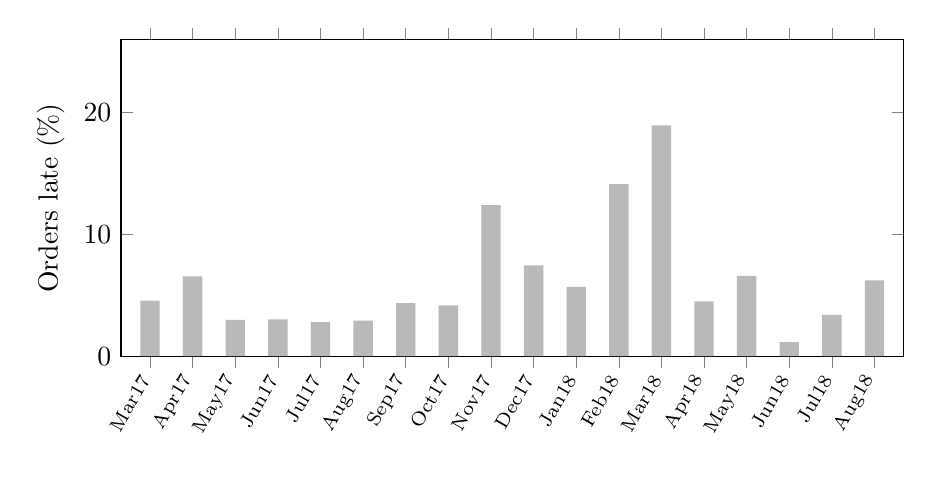
\begin{tikzpicture}
\begin{axis}[width=0.95\linewidth,height=5.6cm,ybar,bar width=7pt,ymin=0,ymax=26,ylabel={Orders late (\%)},
 symbolic x coords={Mar17,Apr17,May17,Jun17,Jul17,Aug17,Sep17,Oct17,Nov17,Dec17,Jan18,Feb18,Mar18,Apr18,May18,Jun18,Jul18,Aug18},xtick=data,x tick label style={rotate=60,anchor=east,font=\scriptsize},
 enlarge x limits=0.04]
\addplot[fill=gray!55,draw=none] coordinates {(Mar17,4.558) (Apr17,6.557) (May17,2.991) (Jun17,3.031) (Jul17,2.799) (Aug17,2.912) (Sep17,4.362) (Oct17,4.176) (Nov17,12.404) (Dec17,7.455) (Jan18,5.701) (Feb18,14.127) (Mar18,18.966) (Apr18,4.506) (May18,6.593) (Jun18,1.157) (Jul18,3.383) (Aug18,6.232)};
\end{axis}
\end{tikzpicture}
% END GENERATED fig_monthly
\caption{Share of orders late by purchase month. Black Friday (November 2017) and February--March 2018 stand out; the final test months on the right were calmer, at \ClsTestLate{}\% late.}
\label{fig:monthly}
\end{figure}


\begin{figure}[H]
\centering
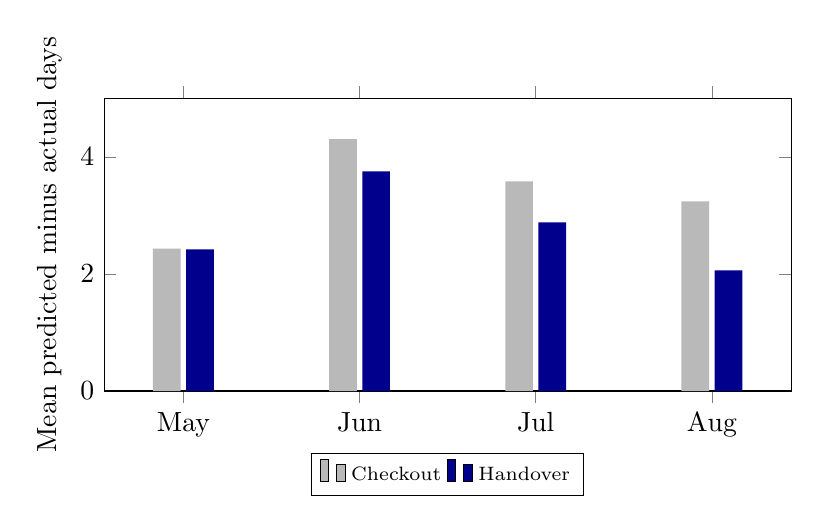
\begin{tikzpicture}
\begin{axis}[width=0.85\linewidth,height=5.3cm,ybar,bar width=10pt,ymin=0,ymax=5,
 symbolic x coords={May,Jun,Jul,Aug},xtick=data,enlarge x limits=0.15,
 ylabel={Mean predicted minus actual days},
 legend style={at={(0.5,-0.21)},anchor=north,legend columns=2,font=\scriptsize}]
\addplot[fill=gray!55,draw=none] coordinates {(May,2.43) (Jun,4.30) (Jul,3.58) (Aug,3.24)};
\addplot[fill=blue!55!black,draw=none] coordinates {(May,2.42) (Jun,3.75) (Jul,2.88) (Aug,2.06)};
\legend{Checkout,Handover}
\end{axis}
\end{tikzpicture}
\caption{Average over-prediction of delivery time by purchase month in the final test period (May starts on the 26th). Positive values mean the model predicted a longer delivery than actually happened, reflecting the shift to faster deliveries. Not used to choose models.}
\label{fig:test-bias}
\end{figure}

% BEGIN GENERATED fig_roc_pr -- refreshed by phase2_final_evidence.py
\begin{figure}[H]
\centering
\begin{minipage}{0.49\linewidth}\centering
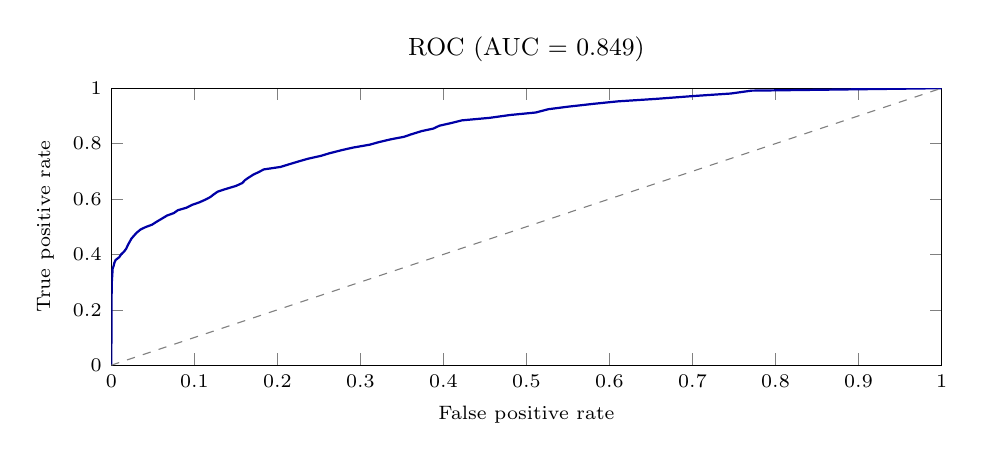
\begin{tikzpicture}
\begin{axis}[width=\linewidth,height=5.1cm,xmin=0,xmax=1,ymin=0,ymax=1,title style={font=\small},tick label style={font=\scriptsize},label style={font=\scriptsize},xlabel={False positive rate},ylabel={True positive rate},title={ROC (AUC = 0.849)}]
\addplot[thick,blue!65!black,no marks] coordinates {(0.0000,0.0000) (0.0003,0.2440) (0.0007,0.3036) (0.0012,0.3274) (0.0016,0.3482) (0.0028,0.3586) (0.0036,0.3690) (0.0051,0.3795) (0.0095,0.3899) (0.0119,0.4003) (0.0155,0.4107) (0.0180,0.4211) (0.0198,0.4330) (0.0220,0.4449) (0.0242,0.4568) (0.0272,0.4673) (0.0303,0.4777) (0.0351,0.4896) (0.0412,0.4985) (0.0491,0.5074) (0.0546,0.5179) (0.0613,0.5298) (0.0671,0.5402) (0.0752,0.5491) (0.0802,0.5595) (0.0904,0.5685) (0.0974,0.5789) (0.1059,0.5878) (0.1137,0.5982) (0.1193,0.6071) (0.1231,0.6161) (0.1281,0.6265) (0.1371,0.6354) (0.1502,0.6473) (0.1578,0.6577) (0.1610,0.6682) (0.1654,0.6771) (0.1707,0.6875) (0.1770,0.6964) (0.1837,0.7068) (0.2039,0.7158) (0.2151,0.7262) (0.2267,0.7366) (0.2371,0.7455) (0.2528,0.7560) (0.2625,0.7649) (0.2781,0.7768) (0.2913,0.7857) (0.3113,0.7961) (0.3220,0.8051) (0.3367,0.8155) (0.3524,0.8244) (0.3611,0.8333) (0.3739,0.8452) (0.3879,0.8542) (0.3952,0.8646) (0.4084,0.8735) (0.4224,0.8839) (0.4555,0.8929) (0.4806,0.9033) (0.5112,0.9122) (0.5264,0.9241) (0.5494,0.9330) (0.5807,0.9435) (0.6099,0.9524) (0.6556,0.9613) (0.7013,0.9717) (0.7461,0.9807) (0.7710,0.9911) (1.0000,1.0000)};
\addplot[thin,gray,dashed,no marks] coordinates {(0,0) (1,1)};
\end{axis}
\end{tikzpicture}
\end{minipage}\hfill
\begin{minipage}{0.49\linewidth}\centering
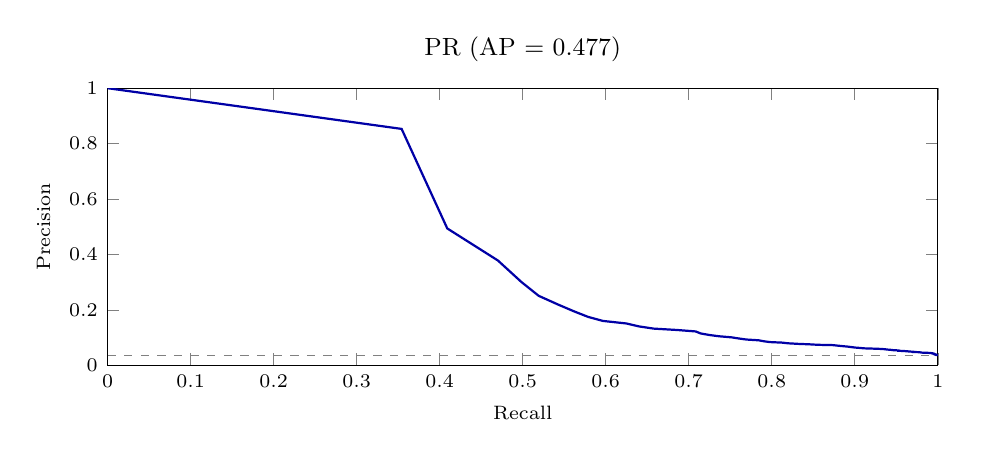
\begin{tikzpicture}
\begin{axis}[width=\linewidth,height=5.1cm,xmin=0,xmax=1,ymin=0,ymax=1,title style={font=\small},tick label style={font=\scriptsize},label style={font=\scriptsize},xlabel={Recall},ylabel={Precision},title={PR (AP = 0.477)}]
\addplot[thick,blue!65!black,no marks] coordinates {(0.0000,1.0000) (0.3542,0.8530) (0.4092,0.4937) (0.4702,0.3780) (0.4985,0.3004) (0.5193,0.2505) (0.5432,0.2183) (0.5625,0.1937) (0.5789,0.1744) (0.5967,0.1599) (0.6250,0.1507) (0.6399,0.1402) (0.6577,0.1322) (0.6860,0.1272) (0.7083,0.1220) (0.7143,0.1148) (0.7247,0.1092) (0.7366,0.1045) (0.7515,0.1007) (0.7604,0.0965) (0.7693,0.0928) (0.7842,0.0900) (0.7902,0.0866) (0.7976,0.0836) (0.8125,0.0816) (0.8199,0.0791) (0.8318,0.0771) (0.8452,0.0755) (0.8557,0.0737) (0.8735,0.0726) (0.8795,0.0707) (0.8854,0.0689) (0.8914,0.0672) (0.8958,0.0655) (0.9003,0.0638) (0.9062,0.0624) (0.9107,0.0610) (0.9211,0.0600) (0.9301,0.0590) (0.9360,0.0579) (0.9390,0.0566) (0.9435,0.0555) (0.9464,0.0543) (0.9524,0.0534) (0.9524,0.0522) (0.9583,0.0514) (0.9628,0.0505) (0.9658,0.0495) (0.9702,0.0487) (0.9702,0.0477) (0.9777,0.0471) (0.9792,0.0463) (0.9807,0.0455) (0.9866,0.0449) (0.9911,0.0443) (0.9926,0.0435) (0.9940,0.0428) (0.9940,0.0420) (0.9955,0.0414) (0.9955,0.0407) (0.9955,0.0400) (0.9970,0.0394) (0.9970,0.0388) (0.9970,0.0382) (0.9985,0.0376) (0.9985,0.0370) (1.0000,0.0365) (1.0000,0.0360) (1.0000,0.0355) (1.0000,0.0349)};
\addplot[thin,gray,dashed,no marks] coordinates {(0,0.0349) (1,0.0349)};
\end{axis}
\end{tikzpicture}
\end{minipage}
\caption{Final handover logistic classifier on 19,230 final-test-period orders (672 late). Curves are sampled points for display; AUC and average precision (AP) use all predictions. Dashed lines show random ranking. The top-\ActShare{}\% review list is drawn separately each month, so it is not a single point on these curves.}
\label{fig:roc-pr}
\end{figure}
% END GENERATED fig_roc_pr

% BEGIN GENERATED fig_confusion -- refreshed by phase2_final_evidence.py
\begin{table}[H]
\centering\small
\caption{Final test period confusion counts for the top-\ActShare{}\% monthly review list. Counts show who would be flagged, before any action is taken.}
\label{tab:app-confusion}
\begin{tabular}{@{}lrr@{}}
\toprule
& Actually late & Actually on time \\
\midrule
Selected for review & 387 & 2,115 \\
Not selected & 285 & 16,443 \\
\bottomrule
\end{tabular}
\end{table}
% END GENERATED fig_confusion

At this list size, MCC is \ClsTestMCC{}, where zero would mean no link between being flagged and being late.

\section{Remedies tested for the August gap}
\label{app:remedies}
These exploratory checks were run after the August gap had been seen. Each was compared on the validation windows before the final period, and none changed the selected model. They use a top-10\% review list, so their counts differ slightly from the main tables; the monthly-retraining check groups lists by handover month and the others by purchase month, so the rule's count differs between them. Code and outputs are in the repository's \texttt{experiments/monthly\_retraining/} and \texttt{experiments/promise\_dependence/} folders.

\begin{table}[H]
\centering\small
\caption{Late orders caught by each remedy against the current model and the remaining-slack rule. $^{*}$On validation, monthly retraining is compared with quarterly retraining; in the final period, with the single model trained in May. ``August short'' counts August orders with promises under \ShortCut{} days that were still before their date at handover (208 late, 336 reviews).}
\label{tab:remedies}
\begin{tabular}{@{}lrrr@{}}
\toprule
Remedy & Validation & Final period & August short \\
& remedy / current & remedy / current / rule & remedy / current / rule \\
\midrule
Monthly retraining$^{*}$ & 1,275 / 1,212 & 375 / 364 / 394 & 67 / 61 / 73 \\
Raw promise inputs removed & 1,321 / 1,315 & 363 / 363 / 398 & 61 / 61 / 73 \\
\quad and promise reconstruction blocked & 1,306 / 1,315 & 362 / 363 / 398 & 58 / 61 / 73 \\
Rule-first model with a bounded correction & 1,314 / 1,315 & 364 / 363 / 398 & 50 / 61 / 73 \\
\bottomrule
\end{tabular}
\end{table}

\section{Full configuration tables}
% BEGIN GENERATED fig_appendix_regression -- refreshed by phase2_final_evidence.py
\begin{table}[H]
\centering\small
\caption{Every regression candidate, mean over five validation windows.}
\label{tab:app-regression}
\begin{tabular}{@{}lllrrr@{}}
\toprule
Stage & Candidate & Family & MAE & RMSE & $R^2$ \\
\midrule
Checkout & mean\_baseline & mean & 7.215 & 10.671 & -0.078 \\
Checkout & linear\_baseline & linear & 5.860 & 9.464 & 0.155 \\
Checkout & ridge\_1 & ridge & 5.858 & 9.462 & 0.156 \\
Checkout & ridge\_10 & ridge & 5.848 & 9.451 & 0.158 \\
Checkout & ridge\_100 & ridge & 5.809 & 9.398 & 0.167 \\
Checkout & tree\_baseline & tree & 7.787 & 12.344 & -0.472 \\
Checkout & tree\_depth6 & tree & 5.933 & 9.505 & 0.144 \\
Checkout & forest\_leaf20 & forest & 5.783 & 9.340 & 0.176 \\
Checkout & boost\_baseline & boost & 5.830 & 9.452 & 0.155 \\
Checkout & boost\_slow & boost & 5.816 & 9.444 & 0.157 \\
Handover & mean\_baseline & mean & 7.215 & 10.671 & -0.078 \\
Handover & elapsed\_plus\_route\_baseline & rule & 5.304 & 8.396 & 0.337 \\
Handover & linear\_baseline & linear & 5.146 & 8.472 & 0.327 \\
Handover & ridge\_1 & ridge & 5.145 & 8.470 & 0.327 \\
Handover & ridge\_10 & ridge & 5.136 & 8.460 & 0.329 \\
Handover & ridge\_100 & ridge & 5.099 & 8.406 & 0.338 \\
Handover & tree\_baseline & tree & 6.840 & 11.625 & -0.330 \\
Handover & tree\_depth6 & tree & 5.313 & 8.633 & 0.299 \\
Handover & forest\_leaf20 & forest & 5.346 & 8.808 & 0.270 \\
Handover & boost\_baseline & boost & 5.214 & 8.651 & 0.297 \\
Handover & boost\_slow & boost & 5.215 & 8.666 & 0.294 \\
Handover & voting\_family\_winners & voting & 5.107 & 8.471 & 0.327 \\
\bottomrule
\end{tabular}
\end{table}
% END GENERATED fig_appendix_regression
% BEGIN GENERATED fig_appendix_classifier -- refreshed by phase2_final_evidence.py
\begin{table}[H]
\centering\small
\caption{Every classifier candidate, mean over five validation windows (handover stage).}
\label{tab:app-classifier}
\begin{tabular}{@{}lrrr@{}}
\toprule
Candidate & PR-AUC & ROC-AUC & Recall at top 10\% \\
\midrule
logistic\_unregularized & 0.354 & 0.736 & 0.341 \\
logistic\_c1 & 0.359 & 0.742 & 0.343 \\
logistic\_c1\_bal & 0.353 & 0.737 & 0.336 \\
logistic\_c0.01 & 0.382 & 0.774 & 0.360 \\
logistic\_c0.01\_bal & 0.372 & 0.764 & 0.349 \\
logistic\_c0.1 & 0.370 & 0.758 & 0.350 \\
logistic\_c0.1\_bal & 0.359 & 0.745 & 0.337 \\
logistic\_c10 & 0.356 & 0.737 & 0.340 \\
logistic\_c10\_bal & 0.350 & 0.733 & 0.333 \\
tree\_plain & 0.137 & 0.559 & 0.208 \\
tree\_d4\_l20 & 0.283 & 0.667 & 0.287 \\
tree\_d4\_l100 & 0.280 & 0.667 & 0.286 \\
tree\_d6\_l20 & 0.303 & 0.693 & 0.313 \\
tree\_d6\_l100 & 0.306 & 0.700 & 0.321 \\
tree\_d8\_l20 & 0.305 & 0.694 & 0.297 \\
tree\_d8\_l100 & 0.308 & 0.684 & 0.322 \\
tree\_d12\_l20 & 0.291 & 0.632 & 0.295 \\
tree\_d12\_l100 & 0.301 & 0.664 & 0.309 \\
forest\_l5\_sqrt & 0.363 & 0.737 & 0.343 \\
forest\_l5\_half & 0.345 & 0.724 & 0.326 \\
forest\_l20\_sqrt & 0.368 & 0.744 & 0.343 \\
forest\_l20\_half & 0.352 & 0.730 & 0.335 \\
forest\_l50\_sqrt & 0.372 & 0.750 & 0.345 \\
forest\_l50\_half & 0.358 & 0.738 & 0.338 \\
boost\_lr0.03\_n200\_l20 & 0.356 & 0.743 & 0.334 \\
boost\_lr0.03\_n200\_l100 & 0.347 & 0.738 & 0.331 \\
boost\_lr0.03\_n500\_l20 & 0.346 & 0.733 & 0.326 \\
boost\_lr0.03\_n500\_l100 & 0.334 & 0.725 & 0.319 \\
boost\_lr0.1\_n200\_l20 & 0.336 & 0.725 & 0.308 \\
boost\_lr0.1\_n200\_l100 & 0.328 & 0.716 & 0.314 \\
boost\_lr0.1\_n500\_l20 & 0.323 & 0.708 & 0.289 \\
boost\_lr0.1\_n500\_l100 & 0.316 & 0.705 & 0.299 \\
\bottomrule
\end{tabular}
\end{table}
% END GENERATED fig_appendix_classifier

\end{document}
